% Answer key for wright-fisher.tex. The figure and the numerical checks of every result
% here are made by scripts/wright_fisher.py. Equation numbers are Gardiner, 2nd ed.
\documentclass[11pt]{article}

\usepackage[letterpaper,margin=1in]{geometry}
\usepackage[T1]{fontenc}
\usepackage{lmodern}
\usepackage{microtype}
\usepackage{amsmath,amssymb,mathtools}
\usepackage[dvipsnames]{xcolor}
\usepackage{graphicx}
\usepackage{enumitem}
\usepackage[most]{tcolorbox}
\usepackage[colorlinks=true,urlcolor=PineGreen,linkcolor=PineGreen]{hyperref}

\graphicspath{{figures/}}
\setlength{\parindent}{0pt}
\setlength{\parskip}{6pt}
\setlist{itemsep=3pt,topsep=2pt}

\newcommand{\dd}{\mathrm{d}}
\newcommand{\avg}[1]{\langle #1\rangle}

\newcommand{\sheethead}[1]{%
  {\sffamily\Large\color{PineGreen}Genetic drift, with and without mutation}\par\vspace{2pt}
  {\sffamily\small Answer key\hfill #1}\par\vspace{-7pt}
  \rule{\textwidth}{0.5pt}\par\vspace{2pt}}
\newcommand{\exsec}[1]{\par\vspace{6pt}{\sffamily\bfseries\large\color{PineGreen}#1}\par\vspace{-2pt}}

\newtcolorbox{keyresults}{enhanced, colback=black!3, colframe=black!35, boxrule=0.4pt, arc=1pt,
  left=6pt, right=6pt, top=4pt, bottom=4pt, colbacktitle=black!10, coltitle=black,
  fonttitle=\bfseries\small, title={Key results}}

\begin{document}

\sheethead{Journal club}

$N$ gene copies, mutation probability $u$ each way per generation, then binomial resampling; $x$ is the fraction of
type $A$, $t$ is in generations, $\theta=2Nu$, and $B$ is the variance per unit time. Equation numbers are Gardiner,
2nd edition.

\begin{keyresults}
\small
\vspace{-6pt}
\begin{alignat*}{2}
  &\text{forward equation:} &\quad& \partial_tp=-\partial_x\bigl[u(1-2x)\,p\bigr]+\tfrac12\partial_x^2\Bigl[\frac{x(1-x)}Np\Bigr] \\
  &\text{stationary state:} &\quad& p_s=\frac{\Gamma(2\theta)}{\Gamma(\theta)^2}\bigl[x(1-x)\bigr]^{\theta-1},\qquad
     H_s=\frac\theta{1+2\theta} \\
  &\text{the end }x=0\text{:} &\quad& \text{regular for }0<\theta<1,\quad\text{entrance for }\theta\ge1,\quad
     \text{exit for }\theta=0;\quad d=2\theta \\
  &\text{with mutation:} &\quad& \lambda_n=\frac{n(n-1+2\theta)}{2N},\quad Q_1=1-2x,\quad
     Q_2=x(1-x)-\frac\theta{2(2\theta+1)};\ \ P_n=p_sQ_n \\
  &\text{without mutation:} &\quad& \lambda_n=\frac{n(n-1)}{2N};\quad Q_0=1,\ Q_1=x;\quad P_n=\frac{Q_n}{x(1-x)}\ (n\ge2) \\
  &\text{decaying modes:} &\quad& P_2=1,\ Q_2=6x(1-x);\qquad P_3=1-2x,\ Q_3=30x(1-x)(1-2x) \\
  &\text{QSD, survival:} &\quad& \text{uniform};\ \ S\simeq6x_0(1-x_0)\,e^{-t/N};\ \
     \frac pS\simeq1+5(1-2x_0)(1-2x)\,e^{-2t/N} \\
  &\text{absorption:} &\quad& \Pr(A\text{ takes over})=x_0,\qquad \avg T_{\rm QSD}=N=1/\lambda_2 \\
  &\text{mean exit time:} &\quad& T(x_0)=-2N\bigl[x_0\ln x_0+(1-x_0)\ln(1-x_0)\bigr],\quad T(\tfrac12)=2N\ln2 \\
  &\text{rare mutation:} &\quad& \frac{p_sQ_2}{\theta/2}\to1-\tfrac12\delta(x)-\tfrac12\delta(x-1),\qquad
     \lambda_1=2u=\text{twice the substitution rate}
\end{alignat*}
\end{keyresults}

% =========================================================
\exsec{(a) Build the forward equation}
Mutation takes $x$ to $x'=x+u(1-2x)$. Resampling gives a new fraction with mean $x'$ and variance $x'(1-x')/N$.
So, exactly,
\[ \avg{\Delta x}=u(1-2x),\qquad \avg{(\Delta x)^2}=\frac{x'(1-x')}N+u^2(1-2x)^2=\frac{x(1-x)}N+O\Bigl(\frac u
   N,u^2\Bigr). \]
With $u=O(1/N)$ the corrections are $O(1/N^2)$, and so are the higher moments. Per generation, $A=u(1-2x)$ and
$B=x(1-x)/N$, so
\[ \partial_tp=-\partial_x\bigl[u(1-2x)\,p\bigr]+\tfrac12\partial_x^2\Bigl[\frac{x(1-x)}N\,p\Bigr],\qquad
   \mathcal L^\dagger f=u(1-2x)\,f'+\frac{x(1-x)}{2N}\,f''. \]
\begin{itemize}
  \item Mutation gives the drift, $A=-2u\,(x-\frac12)$, which pulls $x$ toward $\frac12$ at rate $2u$. Resampling
        is unbiased, $\avg{x_{\rm new}}=x'$, so it contributes only the noise $B$.
  \item A population of one type resamples to that type: there is nothing to sample from, so $B(0)=B(1)=0$.
        Mutation creates the missing type, so $A(0)=u>0$ and $A(1)=-u<0$ point inward.
  \item Both $A$ and $B$ are of order $1/N$, so $x$ changes by order one in order $N$ generations. The natural
        time unit is $N$ generations, and on it only $\theta$ matters.
\end{itemize}

% =========================================================
\exsec{(b) Find the stationary state}
\textbf{1.} $2A/B=2Nu(1-2x)/[x(1-x)]=\theta[1/x-1/(1-x)]$, which integrates to $\theta\ln[x(1-x)]$. Then (5.2.39)
gives $p_s\propto B^{-1}[x(1-x)]^\theta\propto[x(1-x)]^{\theta-1}$, and the Beta integral normalises it:
\[ \boxed{\;p_s(x)=\frac{\Gamma(2\theta)}{\Gamma(\theta)^2}\,\bigl[x(1-x)\bigr]^{\theta-1}\;} \]
Mutation pushes $x$ toward $\frac12$; resampling noise pushes it toward the ends, where it then lingers, because
$B$ is small there. For $\theta>1$ mutation wins and $p_s$ has a hump at $\frac12$. At $\theta=1$ it is flat. For
$\theta<1$ it is U-shaped but integrable: most of the time one type is nearly fixed, until a mutation that
spreads by chance swaps them (figure, panel a).

\textbf{2.} With $x_0=\frac12$ in (5.2.25)--(5.2.28), $f=[4x(1-x)]^{-\theta}$ and
$g=2/(Bf)=2N[x(1-x)]^{-1}[4x(1-x)]^{\theta}$. Near $0$, $f\sim x^{-\theta}$ and $g\sim x^{\theta-1}$.
\begin{itemize}
  \item $0<\theta<1$: $f$ and $g$ are both integrable, so $x=0$ is \textbf{regular}.
  \item $\theta\ge1$: $f$ is not integrable, $g$ is. Then $\int_x^{1/2}f\sim x^{1-\theta}$ (or $\ln(1/x)$ at
        $\theta=1$), so $h_2\sim$ const (or $\ln(1/x)$), which is integrable: \textbf{entrance}.
  \item For later, $\theta=0$: $g\sim1/x$ is not integrable, while $h_1=f\int g\sim\ln(1/x)$ is: \textbf{exit}.
\end{itemize}

\textbf{3.} In the discrete model nothing passes beyond $x=0$, and nothing stays there: a population of type $a$
gains about $Nu=\theta/2$ new $A$ copies per generation, so it leaves $x=0$ within about $2/\theta$ generations,
which is instantaneous on the time scale $N$. So $J(0)=0$, the reflecting condition (5.2.13). A stationary current is the
same everywhere, so $J=0$ throughout, and the zero-current potential solution is the answer. A regular boundary
would also allow stationary states with $J\ne0$, for instance if populations at $x=0$ were removed and restarted
elsewhere. The model rules that out. For $\theta\ge1$ there is no choice: an entrance boundary is never reached.

\textbf{4.} The quick rule sees $B(0)=0$ and $A(0)=u>0$ and says \emph{entrance} for every $\theta>0$. That is wrong
for $\theta<1$. The rule needs $\sqrt B$ to be Lipschitz, and $\sqrt B\simeq\sqrt{x/N}$ is not. Near $0$,
$A\simeq u$ and $B\simeq x/N$. Rescaling $y=4DNx$ gives $\dd y=4DNu\,\dd t+\sqrt{4Dy}\,\dd W$: the squared radius
without the spring, with $dD=4DNu$, so
\[ d=4Nu=2\theta. \]
The talk's thresholds $d=2$ and $d=0$ are $\theta=1$ and $\theta=0$. Near loss, the frequency of $A$ behaves like
the squared distance from the origin of a Brownian particle in $2\theta$ dimensions, which returns to the origin
only in fewer than two dimensions.

% =========================================================
\exsec{(c) Find the eigenfunctions}
\textbf{1.} $\mathcal L^\dagger x^n=\bigl[nu+\tfrac{n(n-1)}{2N}\bigr]x^{n-1}-\bigl[2nu+\tfrac{n(n-1)}{2N}\bigr]x^n$.
So $\mathcal L^\dagger$ is triangular on $1,x,\dots,x^n$. Its eigenvalues are the diagonal entries, and the
eigenvector for each is a polynomial of degree $n$ (they are Jacobi polynomials in $1-2x$):
\[ \boxed{\;\lambda_n=2nu+\frac{n(n-1)}{2N}=\frac{n(n-1+2\theta)}{2N}\;} \]

\textbf{2.} $\mathcal L^\dagger(1-2x)=-2u(1-2x)$, so $Q_1=1-2x$ with $\lambda_1=2u$. Next,
$\mathcal L^\dagger[x(1-x)]=u(1-2x)^2-x(1-x)/N=u-\lambda_2\,x(1-x)$ with $\lambda_2=4u+1/N$. So
$\mathcal L^\dagger[x(1-x)+c]=-\lambda_2[x(1-x)+c]$ requires $c=-u/\lambda_2$:
\[ Q_1=1-2x,\qquad Q_2=x(1-x)-\frac\theta{2(2\theta+1)}. \]

\textbf{3.} $\avg{Q_1(x(t))}=Q_1(x_0)\,e^{-\lambda_1t}$ exactly, which is $\avg x-\frac12=(x_0-\frac12)\,e^{-2ut}$.
Resampling is unbiased, so it scatters $x$ without moving its mean, and only mutation moves the mean. Since
$\lambda_1=2u<\lambda_2$, the gap is the mutation rate itself, however large $N$ is. The discrete chain gives
$(1-2u)^t$ for the same quantity.

\textbf{4.} The stationary current is zero, so (5.2.71)--(5.2.76) apply; the boundary terms vanish because
$Bp_s\sim x^\theta\to0$. With $Q_0=1$, $\int P_2\,\dd x=\int p_sQ_2\,\dd x=\avg{Q_2}_s=0$, so
\[ \avg{x(1-x)}_s=\frac\theta{2(2\theta+1)},\qquad H_s=\frac\theta{1+2\theta}. \]
This agrees with the Beta moment $\theta^2/[2\theta(2\theta+1)]$. Normalised, $P_1=(2\theta+1)\,p_s\,(1-2x)$, since
$\avg{Q_1^2}_s=1/(2\theta+1)$. Because $x=\frac12(Q_0-Q_1)$, its stationary autocorrelation (5.2.90) is a single
exponential: $\avg{x(t)x(0)}_s-\frac14=e^{-2ut}/[4(2\theta+1)]$.

\textbf{5.} $\avg{x(1-x)}$ obeys the closed equation $\frac{\dd}{\dd t}\avg{x(1-x)}=u-\lambda_2\avg{x(1-x)}$.
Resampling destroys diversity at rate $1/N$: two copies share a parent with probability $1/N$ per generation. Mutation
alone would restore it at rate $4u$: $x(1-x)=\frac14(1-Q_1^2)$, and $Q_1^2$ relaxes at $2\lambda_1$. Then
$H_s=2u/\lambda_2$ is the balance of the two, which is the result in 4 again.

% =========================================================
\exsec{(d) Switch off mutation}
\textbf{1.} With $A=0$ the potential solution is $\propto1/B=N/[x(1-x)]$, which is not integrable at either end. So
there is no stationary density. By (b) with $\theta=0$, both ends are \textbf{exit} boundaries: they are reached in
finite time and never left. One type is lost and the other fixed for good. The long-time state is
$(1-\pi)\,\delta(x)+\pi\,\delta(x-1)$, which is not a density on $(0,1)$.

\textbf{2.} $\mathcal L^\dagger x=0$, so $\avg{x(t)}=x_0$ for all $t$: the frequency is a martingale. As
$t\to\infty$, $x\to0$ or $1$, so $x_0=\avg{x(\infty)}=\Pr(A\text{ takes over})$. From (5.2.186)--(5.2.187),
$\frac12B\pi''=0$ with $\pi(0)=0$, $\pi(1)=1$, so $\pi=x_0$. Equivalently, $\psi=1$ in the corrected
(5.2.189)--(5.2.190). A single new mutant, $x_0=1/N$, takes over with probability $1/N$.

\textbf{3.} $\mathcal L^\dagger[x(1-x)]=-x(1-x)/N$, so $\avg{x(1-x)}=x_0(1-x_0)\,e^{-t/N}$: diversity is lost at
$1/N$ per generation. If $\mathcal L^\dagger Q=\frac{x(1-x)}{2N}Q''=-\lambda Q$ and $P=Q/[x(1-x)]$, then
$BP=Q/N$, and
\[ \tfrac12\partial_x^2(BP)=\frac{Q''}{2N}=-\frac{\lambda Q}{x(1-x)}=-\lambda P. \]
The role of $p_s$ is played by $1/[x(1-x)]$, the potential solution of 1, although it cannot be normalised. As in
(5.2.91), which uses the reflecting $p_s$ for absorbing walls, the relation $P=p_sQ$ outlives the stationary state.
So $P_2\propto1$, and
\[ \boxed{\;\text{the QSD is uniform on }(0,1),\qquad P_2=1,\quad Q_2=6x(1-x),\quad
   S(t)\simeq6x_0(1-x_0)\,e^{-t/N}\;} \]
from $\int_0^1x(1-x)\,\dd x=\frac16$. Among populations that still carry both types, every frequency is equally
likely, whatever $x_0$. The odd modes carry no probability, by symmetry, so the next correction to $S$ decays at
$\lambda_4=6/N$.

\emph{The atoms.} $P_2=1$ on $(0,1)$ has total mass $1$ and mean $\frac12$. Biorthogonality with the zero modes
needs $\int P_2\cdot1=0$ and $\int P_2\,x=0$. The full forward mode therefore also has point masses at the ends,
$P_2=1-\frac12\delta(x)-\frac12\delta(x-1)$: what the interior loses, the ends gain, half each. Part (e) meets this
object again.

\textbf{4.} For the QSD $p=1$, $J=-\frac12\partial_x(Bp)=-(1-2x)/2N$. So $J(0)=-1/2N$ flows out through $0$ and
$J(1)=+1/2N$ out through $1$. The total is $1/N=\lambda_2$: a QSD loses probability at its own rate. Write
$J=-\frac12B'p-\frac12Bp'$. Where $B>0$, an absorbing wall needs $p=0$ (5.2.14), and the loss is a diffusive
flux $-\frac12Bp'$. Here $B(0)=0$ and $B'(0)=1/N$, so $J(0)=-p(0)/2N$. The slope of the noise strength acts as a
velocity $-\frac12B'$ that carries probability into the end, and the loss is set by the density there, not its
slope. An exit boundary imposes no condition, so nothing forces $p=0$; the forward equation only requires $p$ to be
integrable.

\textbf{5.} $x(1-x)(1-2x)=x-3x^2+2x^3$ has second derivative $-6(1-2x)$, so
$\mathcal L^\dagger Q_3=-(3/N)Q_3$ and $\lambda_3=3/N$. The partner is $P_3=1-2x$, and normalising gives
$Q_3=30x(1-x)(1-2x)$. Since $P_3$ carries no probability,
\[ \frac{p(x,t)}{S(t)}\simeq1+\frac{Q_3(x_0)}{Q_2(x_0)}\,P_3(x)\,e^{-(\lambda_3-\lambda_2)t}
   =1+5(1-2x_0)(1-2x)\,e^{-2t/N}. \]
The approach rate is $\lambda_3-\lambda_2=2/N$. From $x_0=\frac12$, $Q_3(x_0)=0$ and all odd modes are absent, so
the approach is at $\lambda_4-\lambda_2=5/N$. Here $\lambda_3-\lambda_2=2\lambda_2$: the conditioned density settles
only a little faster than populations are absorbed, so there is no metastability. Panel (b) shows the formula at
work: at $t=N$ from $x_0=0.1$, $p/S\simeq1+0.54(1-2x)$.

\textbf{6.} With $A=0$, (5.2.154) is $\frac{x(1-x)}{2N}T''=-1$, so $T''=-2N[1/x+1/(1-x)]$ with $T(0)=T(1)=0$:
\[ \boxed{\;T(x_0)=-2N\bigl[x_0\ln x_0+(1-x_0)\ln(1-x_0)\bigr],\qquad T(\tfrac12)=2N\ln2\approx1.39N\;} \]
A single mutant is usually lost fast: $T(1/N)\simeq2(1+\ln N)$ generations. Started from the QSD, the interior
density stays uniform and shrinks as $e^{-\lambda_2t}$ exactly. So the absorption time is exponential with mean
$1/\lambda_2=N$, and $\int_0^1T\,\dd x_0=N$. Check: $\int_0^1T\,\dd x=-4N\int_0^1x\ln x\,\dd x=N$.

\begin{figure}[h]
  \centering
  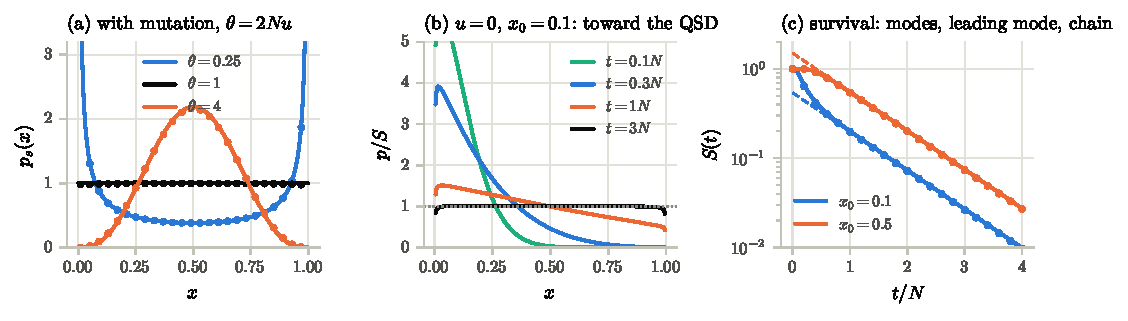
\includegraphics[width=\textwidth]{wf_modes.pdf}
  \caption{\small (a) The stationary density for $\theta=\frac14$, $1$, $4$, with the exact stationary distribution of
  the discrete chain (dots, $N=100$). (b) No mutation, $N=200$, $x_0=0.1$: the chain's distribution, conditioned on
  both types surviving, flattens onto the uniform QSD. The dips at the edges are lattice effects, within a few copies
  of fixation. (c) Survival from $x_0=0.1$ and $\frac12$: mode sum (solid), leading mode $6x_0(1-x_0)e^{-t/N}$
  (dashed), and the chain (dots), $N=200$.}
\end{figure}

% =========================================================
\exsec{(e) Optional: from one to the other}
\textbf{1.} $\Gamma(2\theta)/\Gamma(\theta)^2\simeq(1/2\theta)/(1/\theta)^2=\theta/2$. The probability within
$\varepsilon$ of $0$ is $\simeq\frac\theta2\cdot\varepsilon^\theta/\theta\to\frac12$, while the density in the
interior is $O(\theta)$. So $p_s\to\frac12\delta(x)+\frac12\delta(x-1)$: almost every population is fixed for one
type, each half the time. And $\lambda_1=2u=\theta/N\to0$, so $Q_1=Q_0-2x$ becomes a combination of the two zero
modes of (d), $1$ and the fixation probability $x$. Without mutation, every mixture of the two absorbed states is
stationary; rare mutation picks the even one.

\textbf{2.} $p_sQ_2=\frac{\Gamma(2\theta)}{\Gamma(\theta)^2}[x(1-x)]^\theta-\frac\theta{2(2\theta+1)}\,p_s$. The first
term tends to $\frac\theta2$ on all of $(0,1)$. The second tends to $-\frac\theta2\bigl[\frac12\delta(x)+\frac12
\delta(x-1)\bigr]$. Dividing by $\theta/2$ gives $1-\frac12\delta(x)-\frac12\delta(x-1)$, which is the full $P_2$ of
(d): the uniform QSD inside, and the probability it loses, deposited half at each end. It is orthogonal to
$Q_0=1$ (mass $1-\frac12-\frac12=0$) and to $Q_1=x$ ($\frac12-\frac12=0$). Its rate also matches:
$\lambda_2=4u+1/N\to1/N$.

\textbf{3.} From a population of type $a$, new $A$ mutants arise at rate $Nu$ per generation. Each starts at
$x_0=1/N$ and takes over with probability $1/N$. So the population switches $a\to A$ at rate $Nu\cdot\frac1N=u$, and
$A\to a$ at the same rate. A two-state process with rates $u$ each way relaxes at $u+u=2u=\lambda_1$, which is the
exact gap from (c). The substitution rate equals the mutation rate, independent of $N$: Kimura's neutral rate. It
is the double well of the talk, with the two fixed states as the wells and the gap $\lambda_1\simeq2r$. The picture
needs the time between substitutions, $1/u$, to be much longer than a takeover, which lasts of order $N$
generations, so $\theta\ll1$. Equivalently $\lambda_1=2u\ll\lambda_2\simeq1/N$. For $\theta\gtrsim1$ both types are
usually present (panel a, $\theta=1$ and $4$), and the picture fails, though $\lambda_1=2u$ remains exact.

% =========================================================
\exsec{For the discussion}
\begin{itemize}
  \item \textbf{Two ways to lose a stationary state.} In the talk, the stationary state disappeared when the walls
        were made absorbing. Here no wall changes: switching off mutation turns both ends from regular or entrance
        into exit boundaries. The equation itself decides.
  \item \textbf{Survivors never fix.} Weighting paths by their chance of surviving forever (Doob's $h$-transform,
        with $h=Q_2$) adds the drift $B\,\partial_x\ln Q_2=(1-2x)/N$. That is Wright--Fisher with mutation at
        $\theta=2$. Its stationary density, $\propto x(1-x)=P_2Q_2$, is Beta$(2,2)$, and its ends are entrance
        boundaries ($\theta\ge1$), as they must be.
  \item \textbf{Kimura's solution.} For $u=0$, the interior modes are $P_n=C^{(3/2)}_{n-2}(1-2x)$, Gegenbauer
        polynomials, and $Q_n\propto x(1-x)P_n$. Kimura (1955) found the full transition density this way.
  \item \textbf{Checks.} \texttt{scripts/wright\_fisher.py} builds the transition matrix of the discrete chain. Its
        eigenvalues are exactly $(1-2u)^k\prod_{i<k}(1-i/N)$, whose rates tend to $\lambda_k$. The script checks
        $p_s$, $H_s$ and Feller's test, the residuals of every $Q_n$ and $P_n$ above, and biorthogonality. It
        compares survival from the mode sum with finite differences and with the chain, the fixation probability
        $x_0$, $T(\frac12)$, $\avg T_{\rm QSD}=N$, and the limits in (e).
\end{itemize}

\end{document}
